%!TEX TS-program = xelatex
%!TEX encoding = UTF-8 Unicode

\documentclass{../../../lib/gs}

\usepackage{../../../lib/apf}
\newfontfamily\phonfont{Charis} % font ricco di simboli IPA

% Packages per figure e grafici
\usepackage{pgfplots}
\pgfplotsset{compat=1.18}
\usepackage{tikz}
\usetikzlibrary{decorations.text}
\usepackage{subcaption}

\usepackage{enumitem}

\title{il sogno radicale}
\subtitle{autobiografia di un eretico. appunti revb.\\[1cm] \textbf{\large creazione(opera, operazione)}}
\author{Giuseppe Silvi}
\date{\today}

% Definizione delle parole chiave per i metadati PDF
\kuno{filosofia}
\kdue{greco antico}
\ktre{Platone}
\kquattro{etimologia}
\kcinque{XeLaTeX}

% Comandi per la notazione AllPass
\newcommand{\apf}[3]{\textbf{\texttt{#1(#2,#3)}}}
\newcommand{\apfc}[3]{\begin{center}\apf{#1}{#2}{#3}\end{center}}
\newcommand{\apfcn}[4]{\begin{center}\apf{#1}{#2}{#3}\footnote{#4}\end{center}}

\usepackage[
  backend=biber,
  style=authoryear,        % oppure numeric se preferisci numeri
  sorting=nyt,             % ordina per: nome, anno, titolo
  maxbibnames=3,           % max 3 autori, poi "et al."
  maxcitenames=2,          % in citazione max 2 nomi
  giveninits=false,        % nomi completi, non iniziali
  uniquename=false,
  uniquelist=false,
  url=true,                % mostra URL
  doi=false,               % NON mostrare DOI
  isbn=false,              % NON mostrare ISBN
  eprint=false             % NON mostrare eprint
]{biblatex}

% Personalizzazioni aggiuntive
\DeclareFieldFormat{url}{\newline\footnotesize\url{#1}}
\DeclareFieldFormat{howpublished}{\newline\footnotesize#1}
\DeclareFieldFormat{urldate}{accesso: #1}   % formato data accesso

% Rimuovi completamente i campi che non servono
\AtEveryBibitem{%
  \clearfield{issn}%
  \clearfield{isbn}%
  \clearfield{doi}%
  \clearfield{eprint}%
  \clearfield{eprinttype}%
  \clearfield{pages}% rimuovi se non vuoi vedere le pagine
}

% Per rimuovere "In:" prima del nome della rivista
\renewbibmacro{in:}{}

% Rendi \cite equivalente a \parencite
\let\cite\parencite

% Nel preambolo del .tex
\addbibresource{../../bibliografia.bib}

\usepackage{soul}

% Definizione dello stile per le curve con testo
\tikzset{
  text curve/.style={
    thick,
    postaction={
      decorate,
      decoration={
        raise=-2.4pt,
        text effects along path,
        text align=center,
        text={~#1~},
        text effects/.cd,
          character count=\i,
          character total=\n,
          characters={text along path, fill=white}
      }
    }
  },
  % Stile per la linea base (orizzontale)
  base line/.style={text curve={#1}},
  % Stile per l'arco superiore (da sinistra a destra)
  upper arc/.style={text curve={#1}, ->},
  % Stile per l'arco inferiore (da destra a sinistra, invertito)
  lower arc/.style={
    text curve={#1},
    ->,
    postaction={
      decorate,
      decoration={
        raise=-2.4pt,
        text effects along path,
        reverse path,
        text align=center,
        text={~#1~},
        text effects/.cd,
          character count=\i,
          character total=\n,
          characters={text along path, fill=white}
      }
    }
  }
}

\begin{document}

\maketitle

%-------------------------------------------------------------------------------
\section*{che cos'è opera?}
%-------------------------------------------------------------------------------
Ogni opera è segno. Ogni segno, una volta inciso, è nel passato. L'opera in
quanto segno è discretizzazione di un continuo. Il continuo è granulare. Ogni
opera è segno di segni: segni trapassati in un segno passato, in un segno del
passato. Opera è una relazione di allontanamento.

\begin{figure}[htbp]
\begin{center}
  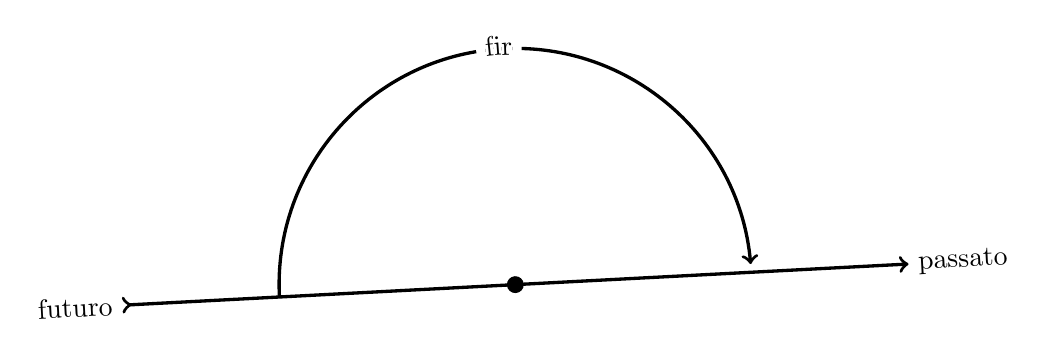
\begin{tikzpicture}
  %  \draw[color=white] (-14.4,-8.2) rectangle (14.4,8.2);
    %\tikzstyle{every node}=[font=\small]

    \begin{scope}[rotate=3]
       \draw[very thick, >->] (-5,0) -- (5,0);
       \draw[upper arc=fir, very thick, ->] (-3,0) arc (180:2:3cm);
  %    \draw[very thick, ->] (3,0) arc (0:-178:3cm);

      % Pallino centrale con etichetta
      \draw[fill=black] (0,0) circle (0.1cm);
      %\node[above=3pt, font=\Large, rotate=3] at (0,0) {$m(t)$};

      % Pallini superiore e inferiore con etichette
  %    \draw[fill=black] (0,3) circle (0.1cm);
  %    \node[above=3pt, font=\Large] at (0,3) {FIR};

  %    \draw[fill=black] (0,-3) circle (0.1cm);
  %    \node[below=3pt, font=\Large] at (0,-3) {IIR};

  \node[anchor=east, rotate=3] at (-5,0) {futuro};
  \node[anchor=west, rotate=3] at (5,0) {passato};
    \end{scope}
  \end{tikzpicture}
%\caption{opera}
\label{opera1}
\end{center}
\end{figure}

L'opera è dunque un momento di crisi del tempo continuo, con determinate
condizioni di risonanza.

Opera è segno.

\section*{che cos'è operazione?}

L'operazione si avvia al primo sintomo di opera, mai prima, mai senza.
L'operazione senza opera è autoscillazione, chiusura al mondo esterno.

L'operazione è un segnale poetico, tendente al futuro. La riattivazione
dell'opera interpretata è un segnale estetico, tendente al passato: è un
trascinare risuonando. L'estetica è nel passato; la poetica preme al futuro.

\section*{che cos'è la loro tensione?}

\begin{figure}[htbp]
\begin{center}
  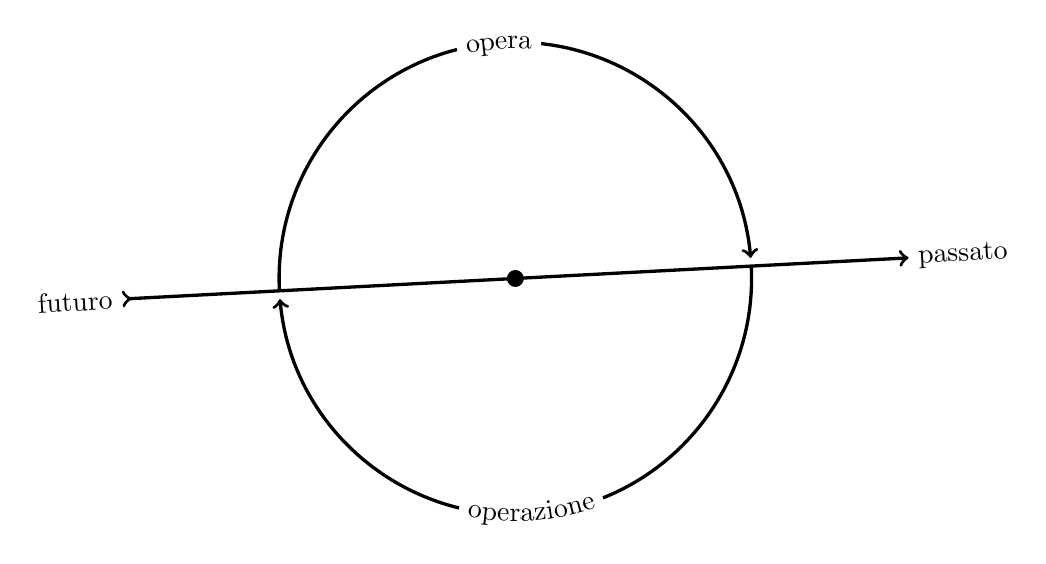
\begin{tikzpicture}
  %  \draw[color=white] (-14.4,-8.2) rectangle (14.4,8.2);
    %\tikzstyle{every node}=[font=\small]

    \begin{scope}[rotate=3]
       \draw[very thick, >->] (-5,0) -- (5,0);
       \draw[upper arc=opera, very thick, ->] (-3,0) arc (180:2:3cm);
      \draw[lower arc=operazione, very thick, ->] (3,0) arc (0:-178:3cm);

      % Pallino centrale con etichetta
      \draw[fill=black] (0,0) circle (0.1cm);
      %\node[above=3pt, font=\Large, rotate=3] at (0,0) {$m(t)$};

      % Pallini superiore e inferiore con etichette
  %    \draw[fill=black] (0,3) circle (0.1cm);
  %    \node[above=3pt, font=\Large] at (0,3) {FIR};

  %    \draw[fill=black] (0,-3) circle (0.1cm);
  %    \node[below=3pt, font=\Large] at (0,-3) {IIR};

  \node[anchor=east, rotate=3] at (-5,0) {futuro};
  \node[anchor=west, rotate=3] at (5,0) {passato};
    \end{scope}
  \end{tikzpicture}
%\caption{opera}
\label{opera1}
\end{center}
\end{figure}

È il senso dell'arte, nei due sensi: $\leftarrow$ poetico; $\rightarrow$ estetico.
Il futuro dell'arte è il non ancora processato. L'operazione tende al futuro. La
loro tensione è creazione, la durata dell'arte. L'arte è l'assoluto dell'opera,
di cui l'opera è discretizzazione, di cui l'operazione è integrazione.


\clearpage

% Nel documento
%\nocite{*}
\printbibliography

\end{document}
